\documentclass{beamer}
\usepackage{textcomp}
\usepackage[utf8]{inputenc}
\usepackage{adjustbox}
\graphicspath{{figures/}}
\setbeamerfont{footnote}{size=\tiny}
\usetheme{Boadilla}
\usecolortheme{seagull}

\usepackage{fancyvrb}
\newenvironment{myverb}{% Verbatim shrinked
 \VerbatimEnvironment
 \begin{adjustbox}{max width=\linewidth}
 \begin{BVerbatim}
  }{
  \end{BVerbatim}
 \end{adjustbox}
}
\title{Differential ChIP-Seq analysis}
\author{\href{mailto:os@jetbrains.com}{Oleg Shpynov}}
\institute{JetBrains Biolabs}

\date{\today}

\begin{document}

\begin{frame}
  \titlepage
\end{frame}

\begin{frame}{ENCODE guidelines summary\footnote{\url{http://encodeproject.org/ENCODE/experiment_guidelines.html}}}
\begin{itemize}
\item Read depth $\geq$ 10 mln reads
\item 2 biological replicates
\item NFR\footnote{This will fail ENCODE guideline, because of new protocol}
\item \textbf{FRiP}
\item Strand cross-correlation
\item NSC for sharp histone modifications 
\item IDR
\end{itemize}
Consensus of 3 peak callers comparison papers:
\begin{itemize}
\item Narrow peaks: MACS2 or SPP \textcolor{gray}{or PeakSe\textbf{g}}
\item Broad and mixed: SICER \textcolor{gray}{or ZINBA or PeakSe\textbf{g}} or RSEG
\end{itemize}
\end{frame}

\begin{frame}{IDR - irreproducible discovery rate}
Given a set of peak calls for a pair of replicate data sets, the peaks can be ranked based on a criterion of significance, such as the P-value, the q-value, the ChIP-to-input enrichment, or the read coverage for each peak.\\
The most significant peaks, which are likely to be genuine signals, are expected to have high consistency between replicates, whereas peaks with low significance, which are more likely to be noise, are expected to have low consistency.\\
A \textbf{major advantage} of IDR is that it can be used to establish a stable threshold for called peaks that is more consistent across laboratories, antibodies, and analysis protocols (e.g., peak callers) than are FDR measures (different for each tool).\footnote{A caution in applying IDR is that it is dominated by the weakest replicate. Additional qc is required}
\end{frame}

\begin{frame}
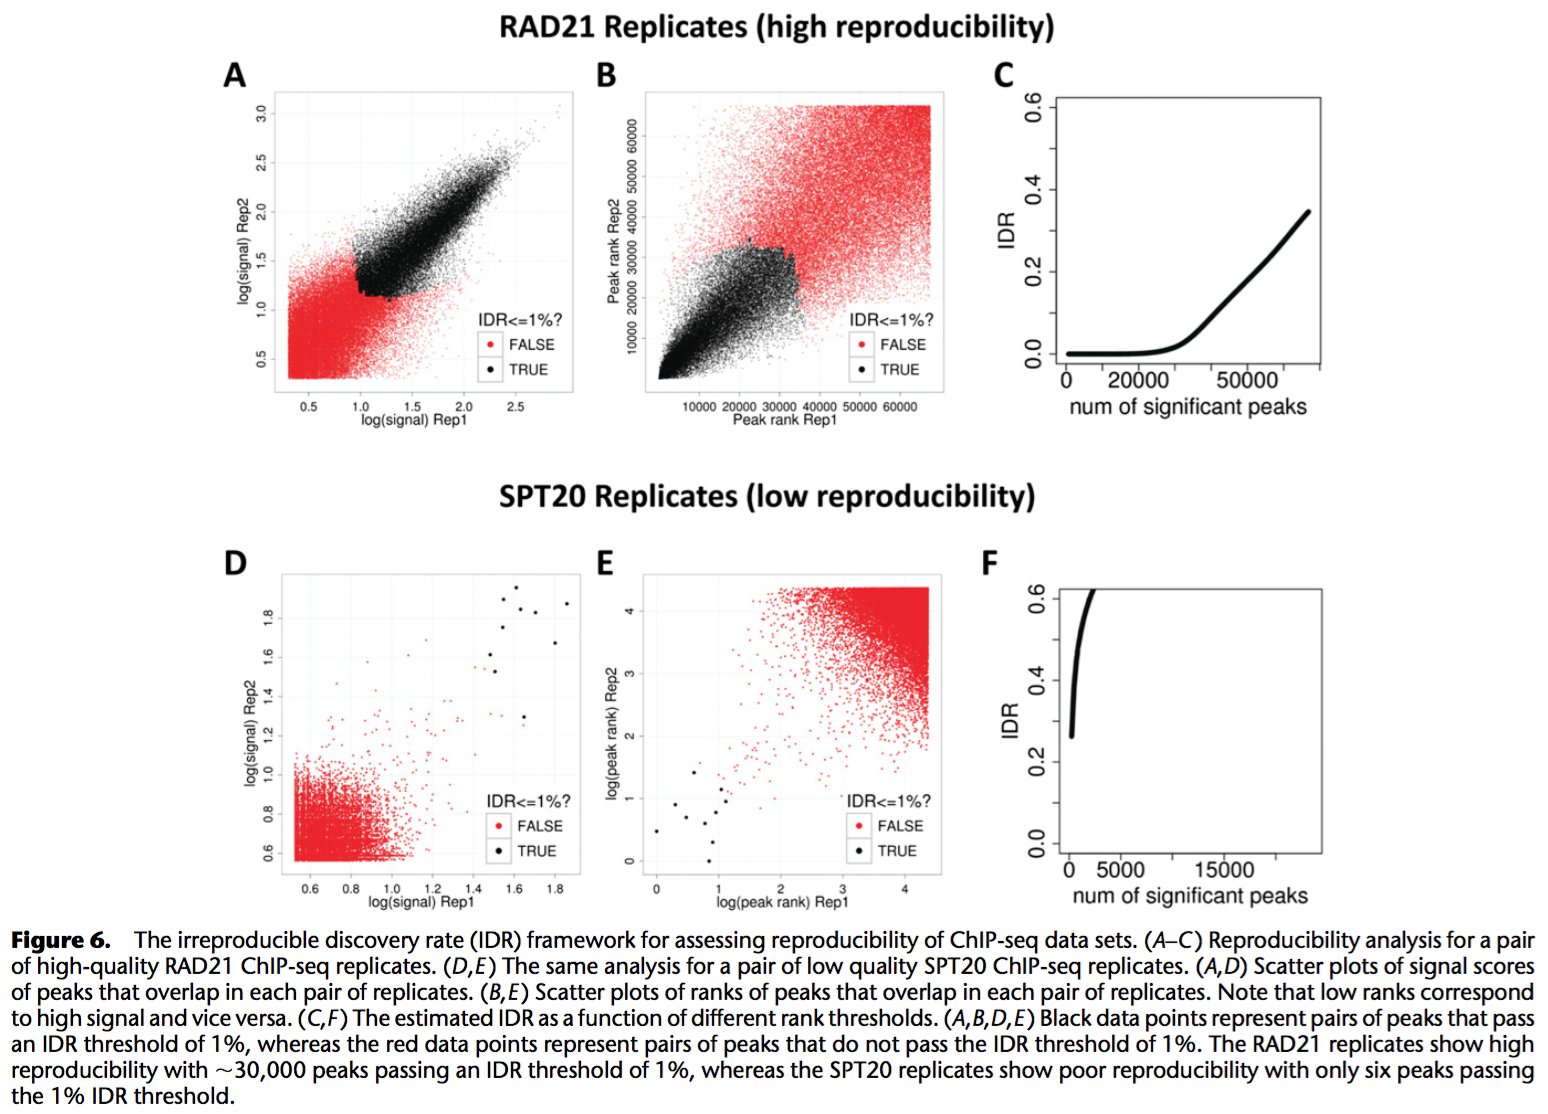
\includegraphics[width=\linewidth]{idr.png}
\end{frame}

\begin{frame}{Differential peak calling}
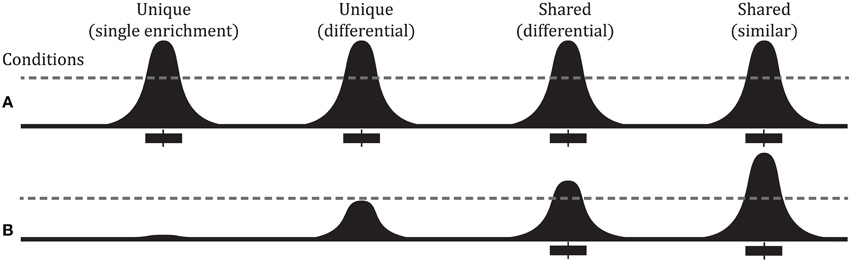
\includegraphics[width=\linewidth]{diff_peaks.jpg}\footnote{Identifying differential transcription factor binding in ChIP-seq}
\end{frame}

\begin{frame}{Differential peak calling}
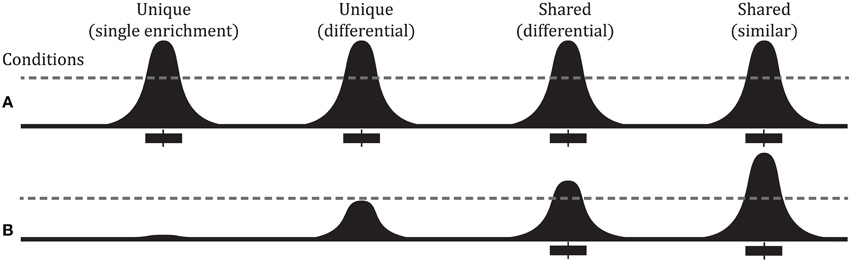
\includegraphics[width=\linewidth]{diff_peaks.jpg}\footnote{\url{http://journal.frontiersin.org/article/10.3389/fgene.2015.00169/full}}
\end{frame}

\begin{frame}{Differential peak calling}
Two alternatives have been proposed.\footnote{Practical Guidelines for the Comprehensive Analysis of ChIP-seq Data}
\begin{itemize}
\item qualitative - hypothesis testing on multiple overlapping sets of peaks\footnote{\url{http://bioinformatics.oxfordjournals.org/content/28/24/3318.short}}.
\item quantitative -  proposes the analysis of differential binding between conditions based on the total counts of reads in peak regions or on the read densities, i.e., counts of reads overlapping at individual genomic positions\footnote{\url{http://www.biomedcentral.com/content/pdf/gb-2010-11-10-r106.pdf}}
\item model based
\end{itemize}
\end{frame}

\begin{frame}{Tools}
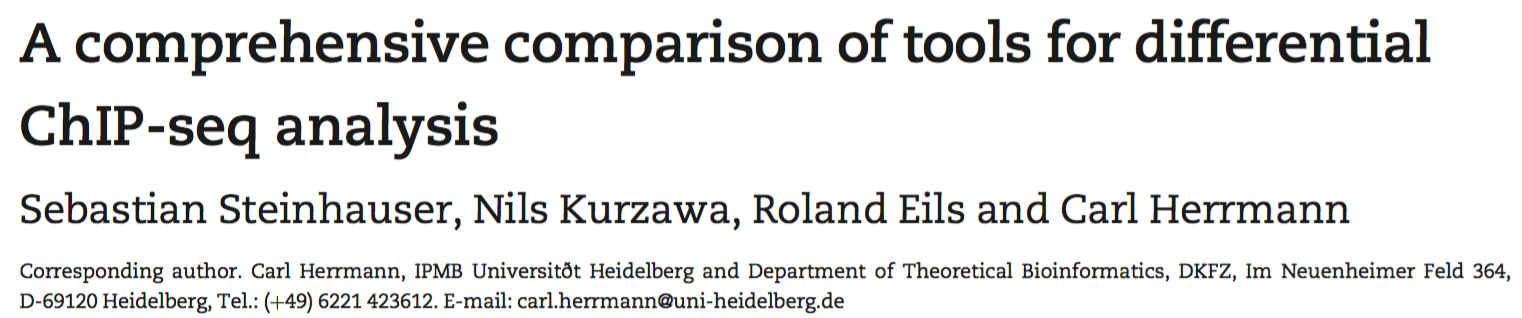
\includegraphics[width=\linewidth]{paperDPC.png}
\end{frame}

\begin{frame}{Problems}
\begin{itemize}
\item  Results obtained by different centers -  systematic bias correction required before data integration can be achieved
\item Reproducibility of the assays is often limited, especially in cases with additional constraints, for example low input material
\item ENCODE project showed that the amount of noise is ${geq}$ 90\% (FRiP)
\item IDR for the rescue!
\end{itemize}
\end{frame}

\begin{frame}{Tools}
 Our criterion for tool selection was the availability of a working software that could be implemented without the need for extensive efforts for porting the code.\footnote{ChipDiff is not there - authors had problems installing it. Indeed.}
\end{frame}

\begin{frame}{Different aims - different approaches - different tools}
Tools
\begin{itemize}
\item Replicated or not
\item ChIPSeq or TF data
\item Control is required or not
\end{itemize}
\end{frame}

\begin{frame}{Test data}
NO gold standard for differential enrichment in ChIP signal.
\begin{itemize}
\item Each category is tested separately, 2 biological replicates for each condition\footnote{Replicates were pooled for single source tools}
\item TF: FoxA1 ChIP-seq for (E2)- and vehicle (Veh)-treated MCF7 (GSE59530) + expression data (GSE59531)
\item Shar ChIP-Seq: H3K27ac for hESC-H1 and mesenchymal stem cells (GSE16256)
\item Broad ChIP-Seq: H3K36me3 for myelome cells TKO vs NTKO (GSE57632)
\item Simulated datasets to estimate Sensitivity/Specificity
\item hg19, BWA, filter out duplicated/bad quality reads
\item MACS2 \\
narrow:  ‘-g hs -q 0.1 –call-summits’\\
broad: ‘-g hs -q 0.1 –broad’
\end{itemize}
\end{frame}

\begin{frame}{Params}
\begin{itemize}
\item NO silver bullet: NO common significant threshold. \\
When possible: FDR $\leq$ 0.01 or P-value $\leq$ 0.05.
\item Gene centric approach: ranked differential peaks by significance - select top 1000 closest genes\footnote{ChIPSeeker}
\item Functional annotation of regions $\pm$ 1.5kb around TSS\footnote{GREAT: single nearest gene}.
\item Jaccard index used as measure of differential peaks correspondence
\item Analyze single tool DR fraction in union of all DR from all tools
\end{itemize}
\end{frame}

\begin{frame}
\centering{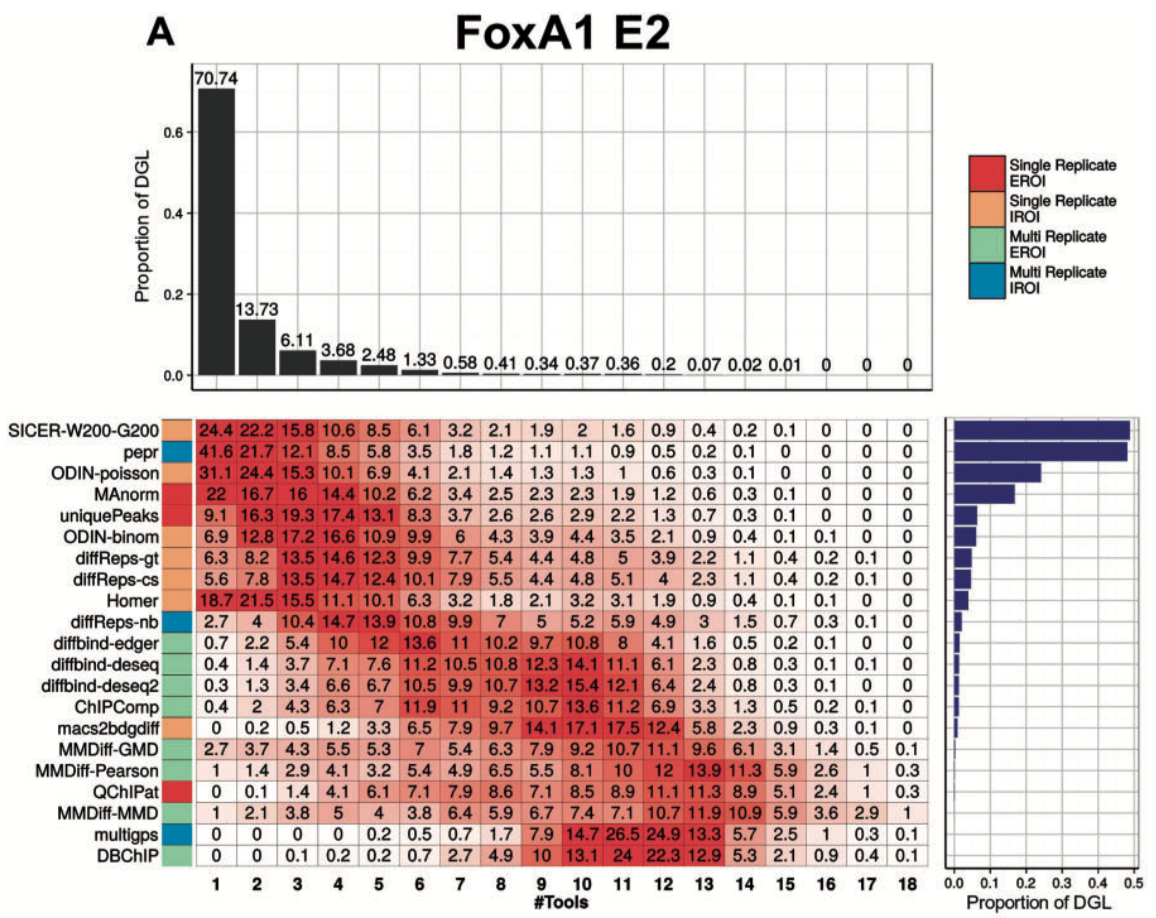
\includegraphics[width=0.9\linewidth]{foxa1.png}}\footnote{EROI/IROI-external regions required\\
Tools - DR is identified by number of tools}
\end{frame}

\begin{frame}
\centering{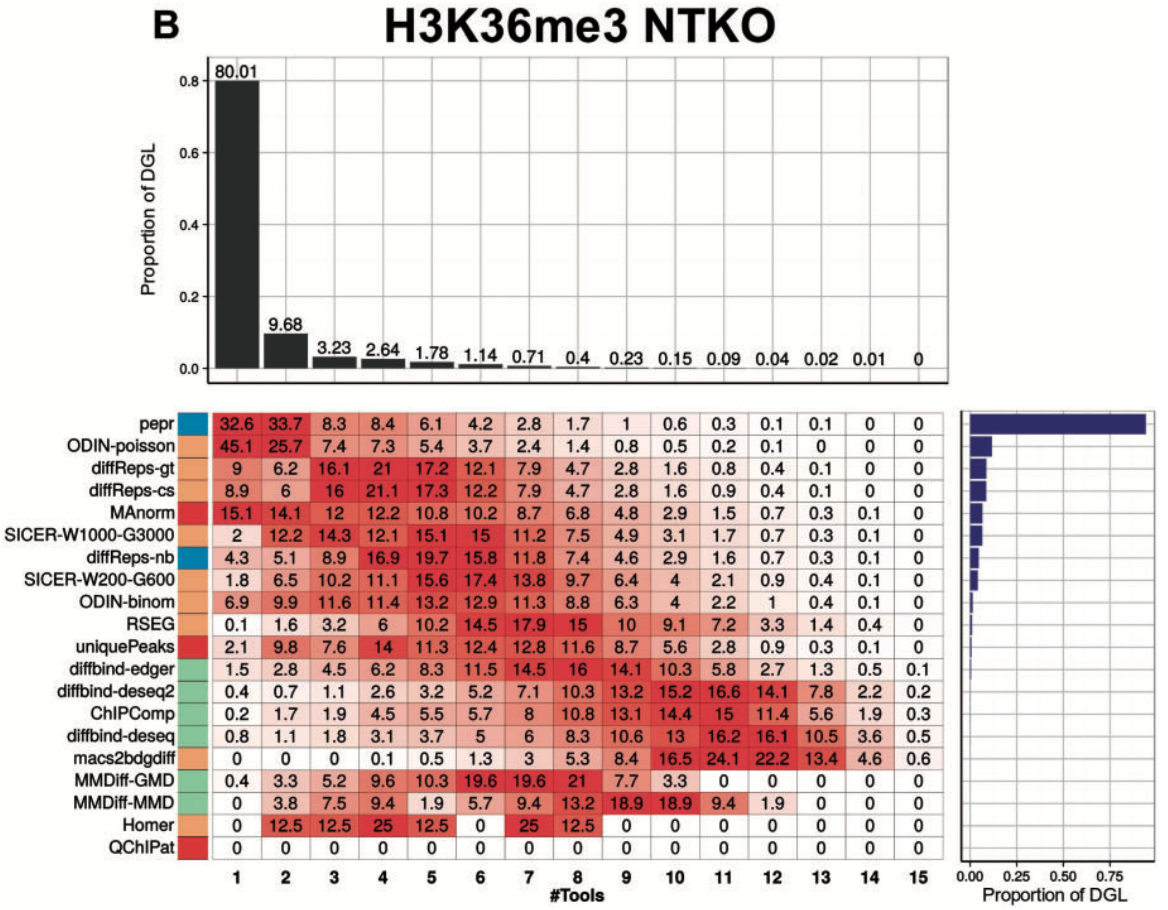
\includegraphics[width=0.9\linewidth]{h3k36me.png}}
\end{frame}

\begin{frame}{Results}
\begin{itemize}
\item Tools for differential ChIP-seq analysis show important differences in the number and size of detected differential regions (DR).
\item Methods taking into account replicates appear to be more robust than those handling single replicate data sets.
\item Inconsistent sets of DR will affect results based on sequence analysis, like detection of enriched transcription factor binding sites.
\item Analysis of functional enrichments based on neighboring genes appears to be more robust.
\item Some tools give good results with default parameters, like ChIPComp or diffBind when replicates are available, or MAnorm, Homer, macs2bdgdiff and RSEG with single replicates. The other tools would require more extensive fine-tuning of parameters to achieve satisfactory results.
\end{itemize}
\end{frame}

\begin{frame}{How do I choose?}
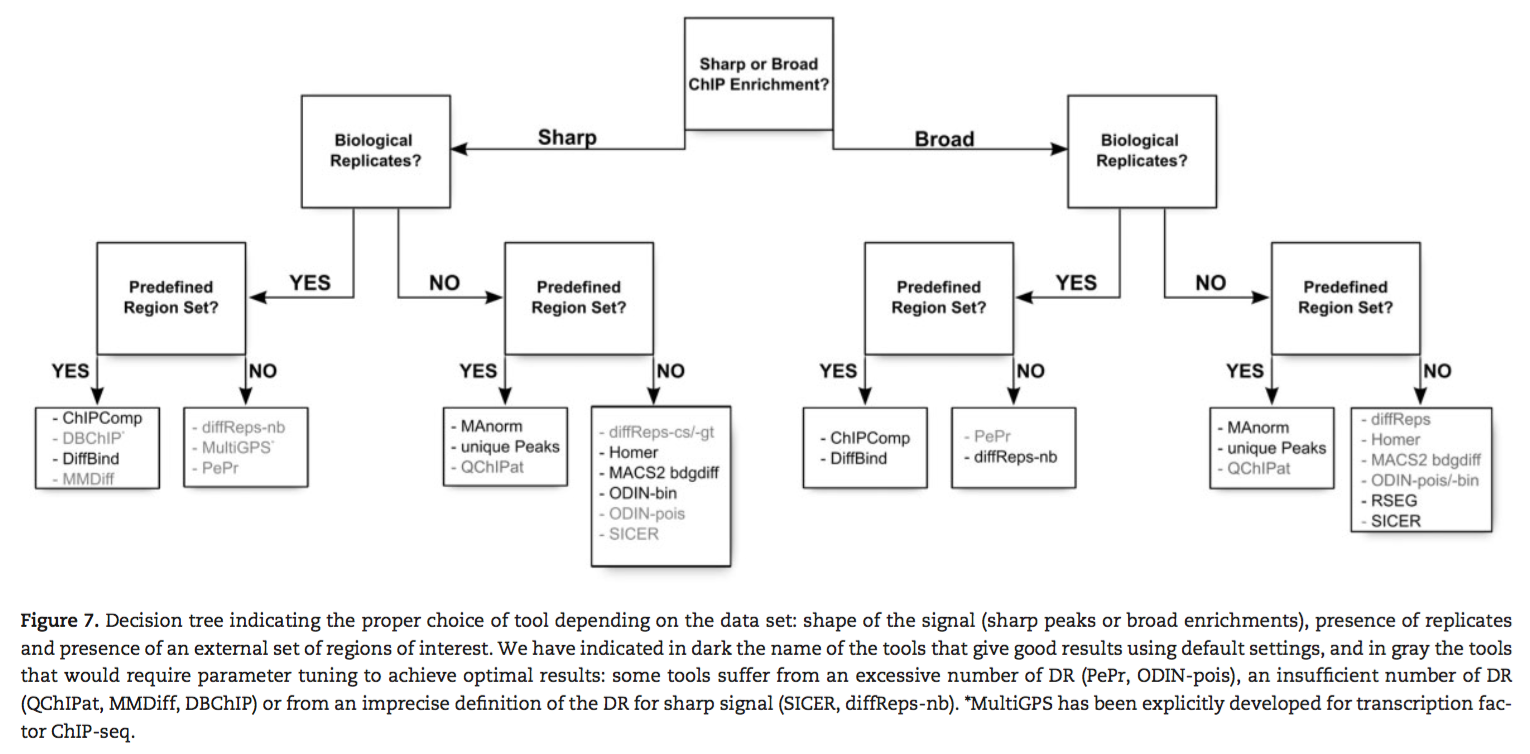
\includegraphics[width=\linewidth]{diffdt.png}
\end{frame}

\begin{frame}{Popular tools}
ChiPDiff\\
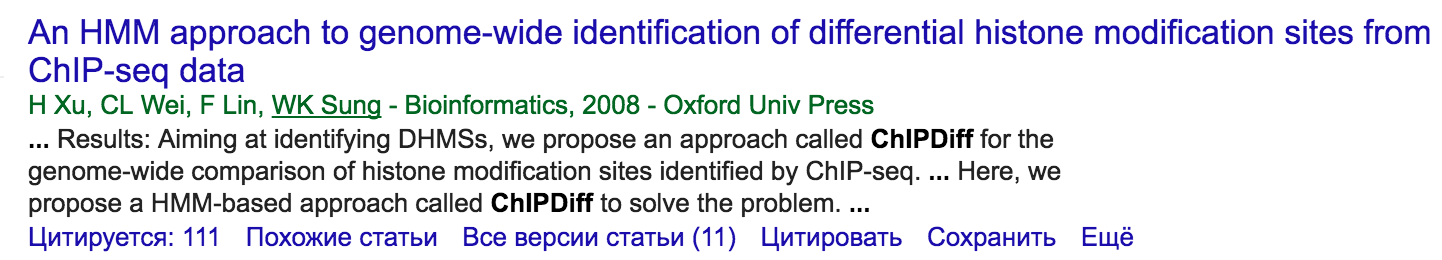
\includegraphics[width=\linewidth]{ChipDiff.png}\\
RSEG\\
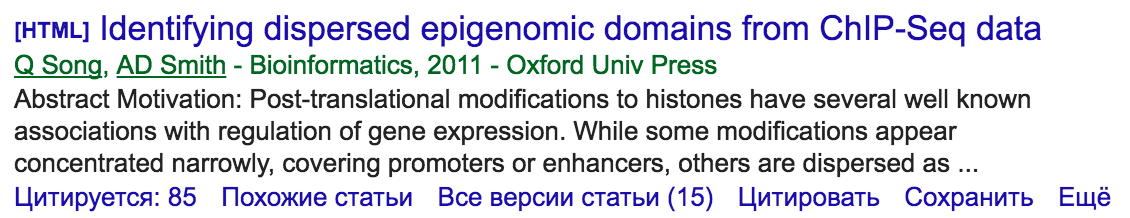
\includegraphics[width=\linewidth]{RSEG.png}\\
MAnorm\\
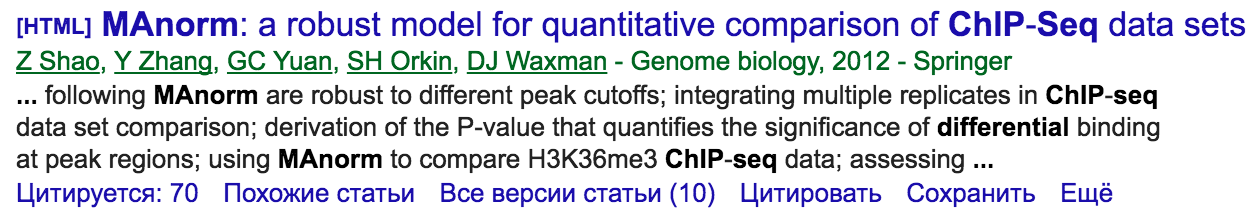
\includegraphics[width=\linewidth]{MAnorm.png}\\
\end{frame}

\begin{frame}{Less popular}
diffReps\\
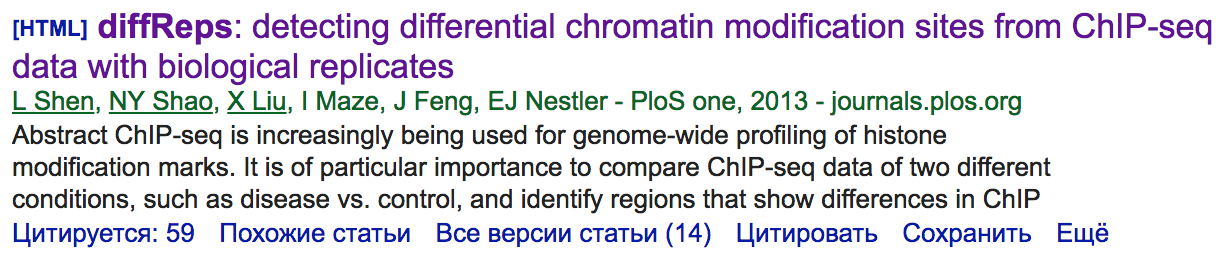
\includegraphics[width=\linewidth]{diffreps.png}\\
DiffBind\\

\includegraphics[width=\linewidth]{DiffBind.png}\\
ODIN\\
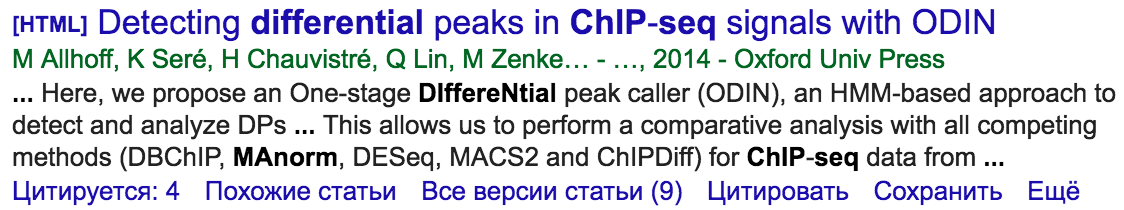
\includegraphics[width=\linewidth]{ODIN.png}\\
\end{frame}
\begin{frame}{Less popular}
ChipComp\\
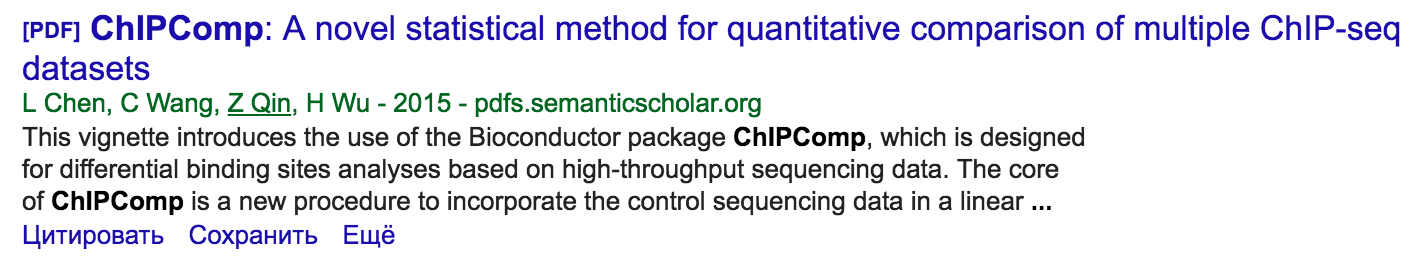
\includegraphics[width=\linewidth]{ChipComp.png}\\
\end{frame}



\begin{frame}
\vspace{4cm}
\centering{
	\huge{Thank you!}
}\\[3cm]
\centering{
	\small{oleg.shpynov@jetbrains.com}\\
	\small{\url{https://research.jetbrains.org/groups/biolabs}}
}
\end{frame}

\end{document}
